\xiti
\begin{xiaotis}
\begin{enhancedline}

\xiaoti{作五边形和已知五边形相位似,相似比为 $k$:}
\begin{xiaoxiaotis}

    \xxt{位似中心取在已知五边形的一边上,它和已知五边形内位似,$k = \exdfrac{4}{3}$,}

    \xxt{取已知五边形的一个顶点为位似中心,它和已知五边形外位似, $k = \exdfrac{3}{4}$。}

\end{xiaoxiaotis}


\xiaoti{如图,四边形 $ABCD$ 和 $A'B'C'D'$ 外位似,相似比 $k_1 = 2$;
    四边形 $A'B'C'D'$ 和 $A''B''C''D''$ 内位似,相似比 $k_2 = 1$。
    四边形 $A''B''C''D''$ 和 $ABCD$ 位似吗?是哪种位似?相似比是什么?
}

\begin{figure}[htbp]
    \centering
    \begin{tikzpicture}
    \tkzDefPoints{0/0/A, 2.5/-0.6/B, 2.3/2.0/C, 1.0/2/D, 3.5/1/O}
    \foreach \n in {A,B,C,D} {
        \tkzDefPointOnLine[pos=0.5](\n,O)  \tkzGetPoint{\n'}
        \tkzDefPointOnLine[pos=2](\n',O)  \tkzGetPoint{\n''}
    }

    \tkzDrawPolygon(A,B,C,D)
    \tkzDrawPolygon(A',B',C',D')
    \tkzDrawPolygon(A'',B'',C'',D'')
    \tkzDrawSegments[dashed](A,A''  B,B''  C,C''  D,D'')
    \tkzLabelPoints[below](A,A')
    \tkzLabelPoints[above](D,C,C',B'')
    \tkzLabelPoints[above=.2em](O)
    \tkzLabelPoints[right](B,B',D'',A'')
    \tkzLabelPoints[below left](D')
    \tkzLabelPoints[below](C'')
\end{tikzpicture}


    \caption*{(第 2 题)}
\end{figure}

\xiaoti{运用位似图形的性质,作已知锐角三角形的内接正方形,使它的一边在已知三角形的一边上,
    另两个顶点分别在已知三角形的其余两边上。
}

\xiaoti{利用放缩尺把一张简易地图放大,使放大图和原图的相似比为 $2:1$。}

\xiaoti{如图的平面图的比例尺是 $1:5000$,根据图中所示的尺寸(单位:厘米),求围墙的长度。}

\begin{figure}[htbp]
    \centering
    \begin{minipage}[b]{7cm}
        \centering
        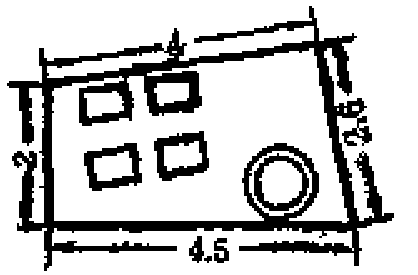
\includegraphics[width=4cm]{../pic/czjh2-ch6-xiti23-05.png}
        \caption*{(第 5 题)}
    \end{minipage}
    \qquad
    \begin{minipage}[b]{7cm}
        \centering
        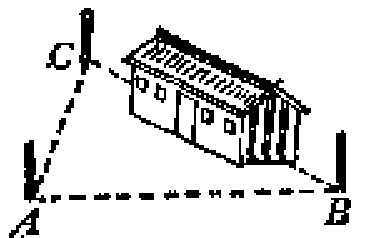
\includegraphics[width=4cm]{../pic/czjh2-ch6-xiti23-06.png}
        \caption*{(第 6 题)}
    \end{minipage}
\end{figure}

\xiaoti{如图,点 $B$ 和 $C$ 之间的距离因有障碍不能直接测量。现测得 $AB = 52$ 米,
    $AC = 44$ 米, $\angle BAC = 42^\circ$。试按 $1:1000$ 的比例尺画出 $\triangle ABC$,
    量出 $BC$ 的长,求出实际距离。
}

\xiaoti{河对岸有目标 $C$。已测得 $AB = 45$ 米, $\angle CAB = 55^\circ$,
    $\angle CBA = 65^\circ$。 用 $1:1000$ 的比例尺画出 $\triangle ABC$,
    量 $AC$、$BC$的长,并求出实际距离。
}

\begin{figure}[htbp]
    \centering
    \begin{minipage}[b]{7cm}
        \centering
        \begin{tikzpicture}[
    river/.style={decorate, decoration={random steps,segment length=3pt,amplitude=2pt}},
]
    \tkzDefPoints{0/0/A, 4.5/0/B}
    \tkzDefTriangle[two angles=55 and 65](A,B)  \tkzGetPoint{C}
    \tkzDrawSegment[thick](A,B)
    \tkzDrawSegments[dashed](A,C  B,C)
    \tkzLabelPoints[left](A)
    \tkzLabelPoints[right](B)
    \tkzLabelPoints[above](C)

    \begin{scope}[yshift=1.1cm]
        \foreach \x in {1, ..., 5} {
            \coordinate (X) at (0, \x/5);
            \draw [river]
                (X) to [out=10, in=160] +(2.5, -0.1)
                to [out=10, in=170] +(5, 0.3);
        }
    \end{scope}
\end{tikzpicture}


        \caption*{(第 7 题)}
    \end{minipage}
    \qquad
    \begin{minipage}[b]{7cm}
        \centering
        \begin{tikzpicture}[
    river/.style={decorate, decoration={random steps,segment length=3pt,amplitude=2pt}},
]
    \tkzDefPoints{0/0/A, 3.9/0/B}
    \tkzDefTriangle[two angles=47 and 80](A,B)  \tkzGetPoint{C}
    \tkzDefTriangle[two angles=87 and 41](A,B)  \tkzGetPoint{D}
    \tkzDrawSegments[thick](A,B  C,D)
    \tkzDrawPolygon[dashed](A,C,B,D)
    \extkzLabelAngel[0.4](B,A,C){$1$}
    \extkzLabelAngel[0.5](C,A,D){$2$}
    \extkzLabelAngel[0.4](D,B,A){$3$}
    \extkzLabelAngel[0.5](C,B,D){$4$}
    \tkzLabelPoints[left](A,D)
    \tkzLabelPoints[right](B,C)

    \begin{scope}[xshift=-.5cm, yshift=1.1cm]
        \foreach \x in {1, ..., 5} {
            \coordinate (X) at (0, \x/5);
            \draw [river]
                (X) to [out=10, in=160] +(2.5, -0.1)
                to [out=10, in=170] +(5, 0.3);
        }
    \end{scope}
\end{tikzpicture}


        \caption*{(第 8 题)}
    \end{minipage}
\end{figure}

\xiaoti{如图,已测得 $AB = 78$ 米, $\angle 1 = 47^\circ$, $\angle 2 = 40^\circ$,
    $\angle 3 = 41^\circ$, $\angle 4 = 40^\circ$。 按 $1:2000$ 的比例尺画出图形,
    量出图中的 $CD$ 的长,求出实际距离。
}

\xiaoti{利用小平板仪测绘操场周围或校园的平面图(用射线法)。}

\end{enhancedline}
\end{xiaotis}

